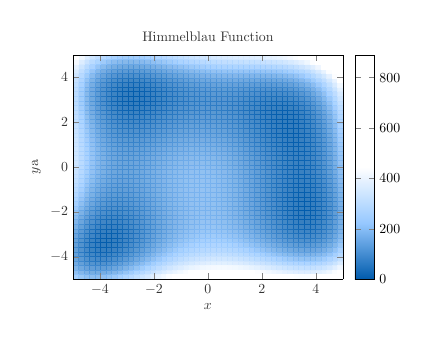
\begin{tikzpicture}[scale = 0.5]
    \begin{axis}[
        colormap={pastel}{ rgb255=(0,91,172) rgb255=(150,200,255) rgb255=(255,255,255)rgb255=(255,255,255)rgb255=(255,255,255)} ,
        view={0}{90},    % Top-down view
        enlargelimits=false,
        axis on top,
        colorbar,        % Add a colorbar
        xlabel=$x$, ylabel=$y$a,
        title={Himmelblau Function},    
        fill opacity=0.8    
    ]
    \addplot3[surf,shader=flat,z buffer=sort,samples=50,domain=-5:5] 
        { (x^2 + y - 11)^2 + (x + y^2 - 7)^2 };
    \end{axis}
\end{tikzpicture}